\section{Discussion} \label{sec:discussion}

We will now describe two experiments evaluating different aspects of
the performance of our algorithm. First, we will look at its running
time on randomly generated domain graphs of different sizes. Second,
we will compare the output of our algorithm to human-generated
descriptions.



\subsection{Quality of Output}

To compare the descriptions generated by our algorithm to
those humans produce, we use a corpus of
human-generated referring expressions collected and made available by
Jette Viethen and Robert
Dale\footnote{http://www.ics.mq.edu.au/~jviethen/drawers}.  The data
was collected in an experiment where participants were asked to
describe one of 16 filing cabinet drawers. The drawers had different
colors and were arranged in a four-by-four grid, as shown in Figure
\ref{fig:drawers}. The human-generated descriptions use four
non-relational properties (the drawer's $\mathsf{color}$, its $\mathsf{column}$ and
$\mathsf{row}$ number, and whether it is in a $\mathsf{corner}$) and five
relational properties ($\mathsf{above, below, next\ to, left\ of,
right\ of}$). Of the 118 referring expressions, only 15 use relational properties.
Viethen and Dale \shortcite{viethen06:_algor_for_gener_refer_expres}
describe the data in more detail and present results of evaluating the
Full Brevity algorithm, the Incremental Algorithm (both by
\cite{Dale1995}) and the relational algorithm by
\cite{dale91:_gener_refer_expres_invol_relat} on this corpus.


\begin{figure}
\begin{center}
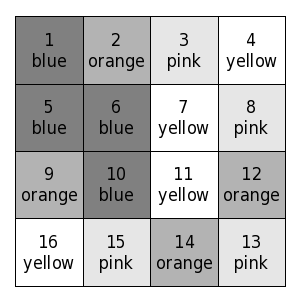
\includegraphics[width=0.25\textwidth]{drawers.png}
\end{center}\vspace*{-3ex}
\caption{A schematic view of the filing cabinets.}\label{fig:drawers}\vspace*{-3ex}
\end{figure}


As described above \todo{needs to be described}, Dale and Reiter's
Incremental Algorithm is a special case of our \el\ algorithm, where
no roles are used and a specific order is imposed on the
predicates. We replicated Viethen and Dale's experiment, which tested
the Incremental Algorithm on the drawer domain with all possible
preference orderings given the four predicates $\mathsf{color, column,
row}$, and $\mathsf{corner}$
\cite{viethen06:_algor_for_gener_refer_expres}.  Unsurprisingly, we
get the same results as they did: 98 of the 103 non-relational
descriptions produced by humans can be generated using one of the 24
possible preference orderings. Unfortunately, there isn't one ordering
that covers all those 98 descriptions - a set of four different
orderings is necessary.



\begin{figure*}[thb]

\begin{small}
\begin{tabular}{|lp{0.9\textwidth}|}\hline
\multirow{2}{*}{drawer} & \textit{human-produce description} \\
& $\mathsf{output\ of\ the\ \el\ algorithm}$\\\hline
2 & \textit{the orange drawer above the blue drawer} \\
& (a) $\exists \mathsf{above}.(\mathsf{blue}) \sqcap \mathsf{orange}$ (b) $\exists \mathsf{above}.(\exists \mathsf{below}.(\mathsf{orange}) \sqcap \mathsf{blue}) \sqcap \mathsf{orange}$ (c) $\exists \mathsf{next}.(\mathsf{blue}) \sqcap \exists \mathsf{next}.(\mathsf{pink}) \sqcap \mathsf{orange}$\\
4 & \textit{the yellow drawer on the top of the pink one} \\ 
& (a) $\exists \mathsf{above}.(\mathsf{pink}) \sqcap \mathsf{yellow}$  (b) $\exists \mathsf{above}.(\mathsf{pink}) \sqcap \mathsf{corner} \sqcap \mathsf{green}$  (c) $\exists \mathsf{above}.(\exists \mathsf{next}.(\mathsf{green}) \sqcap \mathsf{pink}) \sqcap \mathsf{green} \sqcap \mathsf{corner}$\\
5 & $\ast$ \textit{the pink drawer in the fourth column below the yellow one}\\
& (a) $\exists \mathsf{above}.(\mathsf{orange}) \sqcap \mathsf{pink}$  (b) $\exists \mathsf{below}.(\mathsf{green}) \sqcap \mathsf{pink}$  (c) $\exists \mathsf{above}.(\exists \mathsf{next}.(\mathsf{green}) \sqcap \mathsf{orange}) \sqcap \exists \mathsf{next}.(\mathsf{green}) \sqcap \mathsf{pink}$\\
%6 & \textit{the yellow drawer on top of the yellow drawer} / \textit{the yellow drawer that's above another yellow drawer} / $\ast$ \textit{the drawer after the two blue ones in horizontal sequence}\\
6 & \textit{the yellow drawer on top of the yellow drawer} (2$\times$) / $\ast$ \textit{the drawer after the two blue ones in horizontal sequence}\\
& (a) $\exists \mathsf{above}.(\mathsf{yellow}) \sqcap \mathsf{yellow}$  (b) $\exists \mathsf{below}.(\mathsf{pink}) \sqcap \mathsf{green}$  (c) $\exists \mathsf{next}.(\mathsf{blue}) \sqcap \exists \mathsf{next}.(\mathsf{pink}) \sqcap \mathsf{green}$\\
7 & \textit{the blue drawer below the orange one} / $\ast$ \textit{the blue drawer below the orange drawer in the second column}\\ 
& (a) $\exists \mathsf{next}.(\exists \mathsf{above}.(\mathsf{orange}) \sqcap \mathsf{blue}) \sqcap \exists \mathsf{above}.(\mathsf{blue}) \sqcap \mathsf{blue}$  (b) $\exists \mathsf{below}.(\mathsf{orange}) \sqcap \mathsf{blue}$  (c) $\exists \mathsf{next}.(\mathsf{blue}) \sqcap \exists \mathsf{next}.(\mathsf{green}) \sqcap \mathsf{blue}$\\
10 & \textit{the blue drawer above the pink drawer} (2$\times$)\\
& (a) $\exists \mathsf{above}.(\mathsf{pink}) \sqcap \mathsf{blue}$  (b) $\exists \mathsf{above}.(\mathsf{pink}) \sqcap \exists \mathsf{below}.(\mathsf{blue}) \sqcap \mathsf{blue}$  (c) $\exists \mathsf{next}.(\mathsf{orange}) \sqcap \exists \mathsf{next}.(\mathsf{green}) \sqcap \mathsf{blue}$\\
%11 & \textit{the yellow drawer next to the orange drawer} / \textit{the yellow one next to the orange one}\\
11 & \textit{the yellow drawer next to the orange drawer} (2$\times$)\\
& (a) $\exists \mathsf{above}.(\mathsf{orange}) \sqcap \mathsf{yellow}$  (b) $\exists \mathsf{below}.(\mathsf{green}) \sqcap \mathsf{green}$  (c) $\exists \mathsf{next}.(\mathsf{orange}) \sqcap \mathsf{green}$\\
12 & \textit{the orange drawer below the pink drawer}\\ 
& (a) $\exists \mathsf{above}.(\mathsf{pink} \sqcap \mathsf{corner}) \sqcap \mathsf{orange}$  (b) $\exists \mathsf{below}.(\mathsf{pink}) \sqcap \mathsf{orange}$  (c) $\exists \mathsf{next}.(\mathsf{green}) \sqcap \mathsf{orange}$\\
14 & $\ast$ \textit{the orange drawer below the two yellow drawers} (2$\times$)\\
& (a) $\exists \mathsf{next}.(\mathsf{pink} \sqcap \mathsf{corner}) \sqcap \exists \mathsf{next}.(\mathsf{pink}) \sqcap \mathsf{orange}$  (b) $\exists \mathsf{below}.(\mathsf{green}) \sqcap \mathsf{orange}$  (c) $\exists \mathsf{next}.(\mathsf{pink} \sqcap \mathsf{corner}) \sqcap \mathsf{orange}$\\\hline
\end{tabular}
\end{small}

\caption{Human produced descriptions and output of our \el\  algorithm
using the orderings (a) $\mathsf{corner,}$ $\mathsf{color, above,
next, below, right, left}$, (b) $\mathsf{color, corner, below, above,
left, right, next}$ and (c) $\mathsf{corner, color, below}$
$\mathsf{above, left, right, next}$. Descriptions that the \el\
algorithm cannot generate with any ordering are marked by $\ast$.}
\label{fig:example_outputs}
\end{figure*}


% ordering no. 235
%List(corner, green, pink, orange, blue)
%List(above, next, below, right, left)

% ordering no. 19
%List(green, pink, orange, blue, corner)
%List(below, above, left, right, next)

% ordering no. 174
% List(corner, green, pink, orange, blue)
% List(next, above, below, left, right)


\newcite{viethen06:_algor_for_gener_refer_expres} also tested Dale and
Haddock's \shortcite{dale91:_gener_refer_expres_invol_relat}
Relational Algorithm on the drawer domain. Surprisingly, it could not
generate \textit{any} of the descriptions produced by humans. To
evaluate our algorithm's use of relations, we tested it on a
representation of the domain using the predicates $\mathsf{color}$ and
$\mathsf{corner}$ and the roles $\mathsf{above, below, next\ to, left\ of}$,
and $\mathsf{right\ of}$. We did not include the $\mathsf{column}$ and
$\mathsf{row}$ predicates because every drawer can be uniquely
identified through those predicates. Since our algorithm has to
consider predicates before relations, this would mean that no relation
ever gets used. Like for the Incremental Algorithm, we tested all
possible orderings of predicates and roles (with the restriction that
all predicates come before all roles). 10 of the 15 human-produced
descriptions could thus be generated using one of the 240 different
orderings. Figure \ref{fig:example_outputs} shows the output of our
\el\ algorithm for three preference orderings. Together these three
orderings cover 10 of the human-produced descriptions. 
Of the five human-produced escriptions that the \el\
algorithm can not generate, two mention column information, which we
excluded from our domain, and three involve references to sets
(\textit{the two blues ones in horizontal sequence}/\textit{the two
yellow drawers}). While our algorithm cannot reproduce those
descriptions, it does  generate other, simpler descriptions for them.


If we were to use this algorithm in an application, we would of course
have to make a decision on which ordering to use. Dale and Reiter
\shortcite{Dale1995} seem to assume that there is one ordering for a
given domain. The data from the drawer domain do not support this
hypothesis: there is no single ordering that covers all human-produced
descriptions. It is not even the case that one speaker uses only one
ordering in this domain; even though some subjects show a clear trend
towards certain orderings. An interesting open research question is,
therefore, what factors determine which ordering is used. 


To further investigate this question both in the absence and in the
presence of relational properties, we need more human-produced
descriptions using relational properties. The grid structure of the
drawer domain lent itself well to non-relational descriptions using
row and column information and 103 out of 118 human-produced
descriptions are indeed non-relational. The TUNA corpus
\cite{deemter06:_build_seman_trans_corpus_for} used a similar
grid-based mode of presentation and the results are similar in terms
of the number of relational descriptions used. However, many domains
do not have such an internal structure which makes the use of
relations unnecessary. We are currently preparing an experiment to
collect referring expression data similar to the drawer corpus but
using a blocks world domain that will hopefully






\subsection{Efficiency}

Both the \el\ and the \alc\ algorithms took about 15 milliseconds to
compute distinguishing concepts for all 16 individuals in the Viethen
\& Dale dataset.\footnote{We measured all runtimes on a MacBook Pro
  (Intel Core 2 Duo, 2.16 GHz) running Java 1.6 beta, and allowed the
  Java VM to warm up, i.e.\ just-in-time compile all bytecode, before
  taking the measurements.}

\begin{figure}[thb]
  \centering
  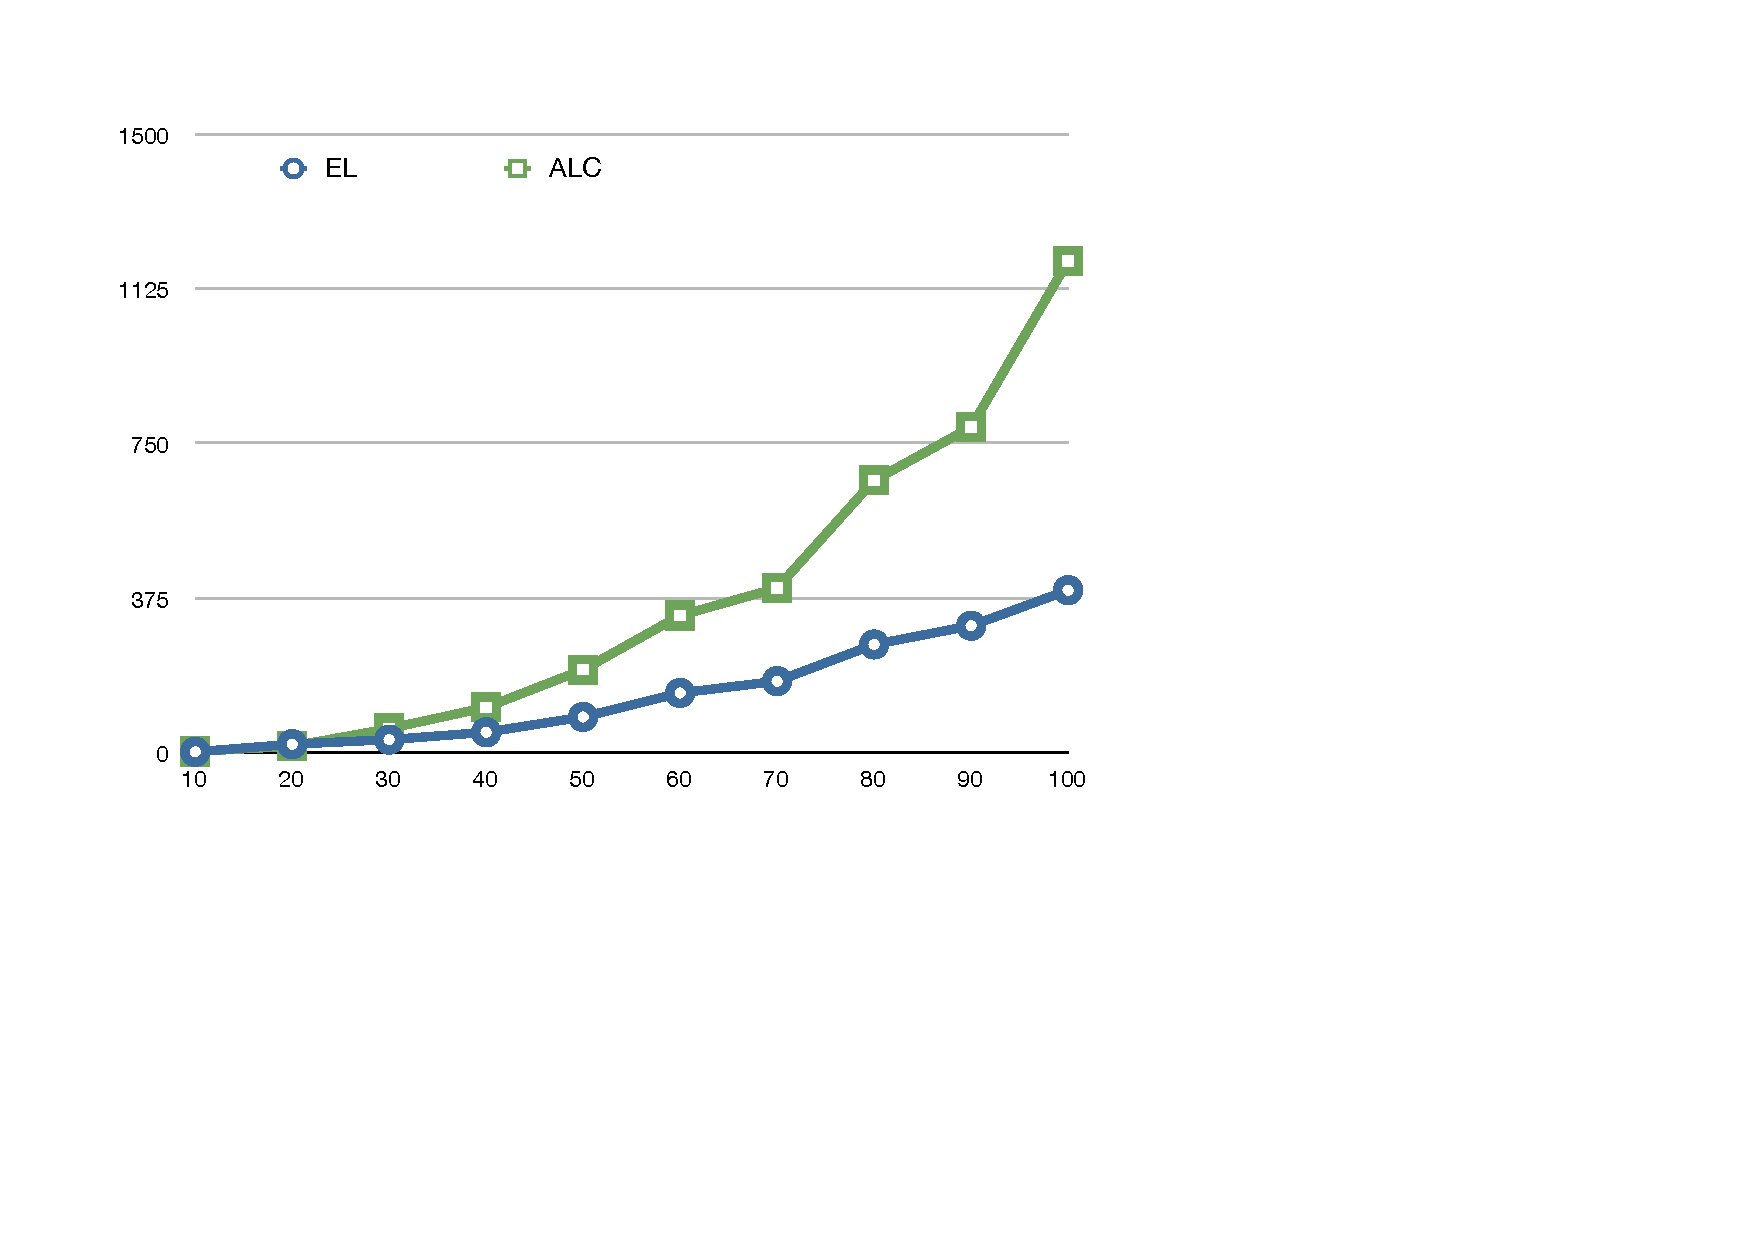
\includegraphics[width=\columnwidth]{runtimes}
  \caption{Average runtimes (in ms) of the two algorithms on random
    models of     different sizes.} 
  \label{fig:runtimes}
\end{figure}

In order to get a more comprehensive picture of the algorithms'
efficiency, we ran them on random models with increasing numbers of
individuals.  Each model had random interpretations for ten different
propositional and four relational symbols; each individual had a 10\%
chance to be in the extension of each propositional symbol, and each
pair of individuals had a 10\% chance to be related by a relational
symbol.  The results (averaged over 10 runs for each model size) are
shown in Fig.~\ref{fig:runtimes}.  As the figure shows, the \el\
algorithm takes about 350 ms on average to generate relational REs for
all individuals in the model of size 100, i.e.\ less than 4 ms on
average for each individual.  The \alc\ algorithm is even faster, at
about 140 ms for the model of size 100.  As far as we know, these are
by far the fastest published runtimes for any relational GRE algorithm
in the literature.

Another encouraging aspect of both runtime graphs is that they seem to
be approximated well by quadratic functions.  So although the
worst-case runtime of the \el\ algorithm might be exponential, both
algorithms empirically exhibit (low) polynomial runtime on the inputs
we considered.



\subsection{Interface to realization}

%\begin{itemize}
%\item there's a risk to generate a concept that can't be realized,
%  especially for the \alc\ algorithm
%\item everybody except perhaps SPUD has this problem
%\item problem is worse in our case because it is harder to control the
%  order in which atoms and relations are explored
%\item would be interesting for future work to think about how
%  search in the bisim algorithms can be controlled by the realizer
%\end{itemize}

Our GRE algorithms do not guarantee that the concepts they compute can
actually be realized in language.  For example, none of the concepts
our algorithms computed in the Viethen \& Dale domain contained an
atom that would commonly be realized as a noun; the property
$\mathsf{drawer}$ is never used because it applies to all individuals
in the domain.  This particular problem could easily be worked around
in a post-processing step.  However, another problem arises from the
massive use of negation in the \alc\ algorithm; it will be hard for
any realizer to find a reasonable way of expressing the concept $\neg
\exists R.(\neg P \sqcap \neg Q)$ from the example in
Fig.~\ref{fig:el-vs-alc} as a smooth noun phrase.  Although we agree
with \newcite{deemter01:_gener_refer_expres} and others that the
careful use of negation and disjunction can improve REs, these
connectives must not be overused.  Thus we consider the concepts
computed by the \el\ algorithm ``safer'' with respect to realization.

Of course, we share the problem of interfacing GRE and realization
with every other approach that separates these two modules, i.e.\
almost the entire GRE literature (notable exceptions are e.g.\ SPUD
\cite{Stone2003a} and \newcite{Horacek1997}).  In principle, we
believe that it is a good idea to handle sentence planning and
realization in a single module; for instance, SPUD can use its
awareness of the syntactic context to generate succinct REs as in
``take the rabbit from the hat''.  We hope that the ideas we have
explored here for efficient and expressive RE generation can
eventually be combined with recent efficient algorithms for integrated
sentence planning and realization, such as in \newcite{KolSto07}.

One problem that arises in our approach specifically is that the
bisimulation classes algorithms derive some measure of efficiency from
their freedom to build concepts without having to respect any
linguistic constraints.  It seems straightforward to extend Krahmer et
al.'s \shortcite{Krahmer2003} approach such that it only considers
subgraphs that can actually be realized, because their algorithm
proceeds by a genuine search for uniquely identifying subgraphs, and
will simply take a different branch of the search if some subgraph is
useless.  Our algorithms don't search in the same way; any constraints
that disallow certain refinements of a partition jeopardize the
algorithms' ability to find a partition into singletons in polynomial
time.  A particularly vivid example is the fact that both algorithms
crucially split over all propositional symbols before they start
iterating over relational symbols; changing this may make them
incomplete.  Investigating this interplay between efficiency and
linguistic constraints is an interesting avenue for future research.




%%% Local Variables: 
%%% mode: latex
%%% TeX-master: "dl-gre-08"
%%% End: 
